\section{Additional results for \texorpdfstring{Section~\ref{sec:frm}}{Section 7}: formation}\label{sup:frm}

This section collects statements, examples and remarks of \cref{sec:frm} that the main text cites without stating in full. Proofs are in \cref{app:frm}.

\subsection{Status summary from the section opening}\label{sup:frm-status-summary-from-the-section-opening}

The result is partial. In the two-group model at $\gamma=\infty$ with noiseless angle observations, $\sigma_\alpha^2=0$, clauses (T1) to (T3) and (T5) of \cref{def:frm-target} are theorems, the contrast clause (T3) at the levels of the window of \cref{thm:frm-split-contrast}(c), which is nonempty at every computed parameter point (\cref{obs:frm-grid}), and the declared start is then itself the split (\cref{thm:frm-formation}(e), \cref{thm:frm-split-contrast}). For $\gamma_S<\gamma<\infty$ reachability of the split branch is a theorem about the frozen-calibration mean-field map (\cref{thm:frm-formation}(a),(b)), with the stochastic-approximation step from the full model to the map open (\cref{open:frm-closure}), and the contrast of the reached state is computed at the base point (\cref{obs:frm-exploration}). Clause (T4) fails for the translation-aware null of type S from a start law that is exchangeable given the world path, as the declared start with identical initial beliefs is, so from such a start the model yields no formation result in the sense of \cref{def:frm-target}. Formation there is a calibration-level effect of misreading joint structure: receivers that know their translation errors pay no mistranslation cost, so from a start law exchangeable given the world path the model's collectives fail the translation-aware form of the exact-fusion persistence clause of the null family, as \cref{prop:frm-exact-fusion} proves, while for full cross-covariance-aware exact fusion in this model the conclusion is heuristic; above a threshold $\gamma_T$ they coincide with the code partition. The split differs from the deletion nulls by proof, and from the frozen-environment null only when the initial states that frozen messages carry are deterministic or conditioned on (\cref{prop:frm-nulls}(a)). Persistence under exact fusion with drifting frames is a conjecture (\cref{conj:frm-drifting-frames}). Online calibration from a symmetric start reaches the split's attention pattern (not necessarily a split selected by contrast) in 0 to 7 of 8 replicates per cell, with reruns of a cell differing by up to three replicates, and is open (\cref{obs:frm-online,open:frm-online}). Formation beyond this model is a conjecture (\cref{conj:frm-formation}).

\subsection{Two mechanisms: flattening and bistability}\label{sec:frm-mechanisms}

Two facts make formation plausible before a population is modeled: grounded learning corrects translations only on attended edges, and attention follows calibrated precision, which learning raises.

\begin{proposition}[Grounded learning flattens the attended subgraph]\label{prop:frm-flattening}
Let codes have full rank, and suppose that every learned translation $\Theta_{ij}(t)$ (\cref{sec:fw-frames}) converges, with limit $U_iU_j^{-1}$ on the event that receiver $i$ attends sender $j$ infinitely often with grounding. Then on the event that the limiting holonomy of a cycle (\cref{thm:coh-holonomy}) differs from the identity, some edge of the cycle is attended only finitely often: the subgraph of edges attended infinitely often is asymptotically flat.
\end{proposition}
% src: L3-P15 (stated here for full-rank codes; the rank-limited version also needs the identifiable subspaces to be carried into one another along the cycle)
\begin{proof}
If every edge of a cycle $i_0,i_1,\dots,i_L=i_0$ is attended infinitely often, each $\Theta_{i_{l+1}i_l}$ converges to $U_{i_{l+1}}U_{i_l}^{-1}$, and by continuity of matrix products the holonomy $\Theta_{i_0i_{L-1}}\cdots\Theta_{i_1i_0}$ converges to $U_{i_0}U_{i_{L-1}}^{-1}\cdots U_{i_1}U_{i_0}^{-1}=I$.
\end{proof}

The hypothesis holds for grounded least squares at full rank (\cref{prop:fw-rls}) and fails for a learner that regresses on an attenuated code (\cref{prop:fw-grounded-identification}(c)). Persistent inconsistency thus sits on edges that end up unattended, the consistency part of hypothesis H3. Which edges these are depends on attention and learning together; in the simplest instance one receiver of capacity one chooses each round between an in-group sender, read correctly, and a cross sender whose frame drifts, in the static model of \cref{def:coh-calibration-model} with C1g calibration. Let $\mathcal A(\mathsf p)$ be the believed value (\cref{def:mis-values}) of the cross sender minus that of the in-group sender when the cross sender is attended with frequency $\mathsf p$, in the expected-variance mean field of grounded angle learning (\cref{app:frm}); attention feeds learning, so $\mathcal A$ is continuous and strictly increasing on $(0,1]$ with a finite limit $\mathcal A(0)$. With $[\cdot]$ the indicator of a statement, attention at policy precision $\gamma$ follows $\mathsf p=1/(1+e^{-\gamma\mathcal A(\mathsf p)})$, and at $\gamma=\infty$ it follows $\mathsf p=[\mathcal A(\mathsf p)>0]$.

\begin{proposition}[Bistability of attention and learning]\label{prop:frm-bistability}
In the single-edge mean field at $\gamma=\infty$ let the attention frequency relax toward the attention rule, $\dot{\mathsf p}=[\mathcal A(\mathsf p)>0]-\mathsf p$. The split state $\mathsf p=0$ is an attracting rest point if and only if $\mathcal A(0)<0$, and the merged state $\mathsf p=1$ is one if and only if $\mathcal A(1)>0$. When $\mathcal A(0)<0<\mathcal A(1)$ both attract, and the unique root $\mathsf p^\dagger$ of $\mathcal A$ separates their basins.
\end{proposition}
% src: L3-P16 part 1 (the expected-variance mean field is declared as the model); part 2 as the computed instance
Proof in \cref{app:frm}. The mean field replaces the random variance recursion of intermittent observation by its expected value. An unattended edge is never learned and stays unattractive, so a cut reinforces itself and the outcome depends on initial attention. At finite $\gamma$ exploration of order $e^{-\gamma|\mathcal A(0)|}$ competes with the cut: in a computed instance there is one fixed point, merged, for $\gamma\le50$ and three for $\gamma\ge80$ (\cref{chk:frm-bistability}).

\subsection{Status summary after the mean-field theorem}\label{sup:frm-status-summary-after-the-mean-field-theo}

\Cref{thm:frm-formation} concerns the frozen-calibration mean-field map; the step from the full model to the map is open (\cref{open:frm-closure}). The split branch it reaches is a calibration-level effect of misreading joint structure, and above $\gamma_T$ it coincides with the code partition. That the blocks of the split are collectives is a theorem only at $\gamma=\infty$ with $\sigma_\alpha^2=0$ (\cref{thm:frm-split-contrast}) and a computation at the base point for finite $\gamma$ (\cref{obs:frm-exploration}). From a start law exchangeable given the world path the split fails the translation-aware form of the exact-fusion persistence clause, as \cref{prop:frm-exact-fusion} proves; for full cross-covariance-aware exact fusion this conclusion is heuristic (\cref{sec:frm-fails}). Persistence with drifting frames and formation beyond the model are conjectures (\cref{conj:frm-drifting-frames,conj:frm-formation}), and online calibration from a symmetric start reaches the split's attention pattern (not necessarily a split selected by contrast) in only 0 to 7 of 8 replicates per cell, with reruns of a cell differing by up to three replicates (\cref{obs:frm-online,open:frm-online}).

\subsection{Fixed points, thresholds and bridged states}\label{sup:frm-fixed-points-thresholds-and-bridged-stat}

\begin{observation}[Fixed points and thresholds at the base point]\label{obs:frm-thresholds}
At the base point $\mathsf p^\ast=0.0503$, $\Delta\mathcal V(\frac12)=0.0592$ and $\Delta\mathcal V_{\max}=0.313$, so $\gamma_S=68.2$ and $\gamma_M=6.84$; the symmetric fixed points are those of \cref{tab:frm-thresholds}. Continued in $\gamma$, they form a merged and a split branch joined by an unstable middle branch through folds at $\gamma=60.05$ and $105.9$. The merged branch loses stability to symmetry-breaking perturbations at $\gamma=87.9$, before its fold: for $87.9<\gamma<105.9$ its symmetry-breaking multiplier lies between one and $1.026$, its value at the fold. The split branch is stable from $\gamma=60.11$. Conditions (i) and (ii) of \cref{thm:frm-formation}(b) fail at $\gamma=240$ and hold at $244$ and every larger value computed, while a single learned bridge survives at $240$, so (b) is sharp to within 2 percent here. Computed by bisection, $\gamma_T=242.1$ at the base point, and $\gamma_T=244.2$, $861.1$, $3255.6$ and $12684$ at $\mathsf p^\ast=0.05$, $0.025$, $0.0125$ and $0.00625$ (varied through $h$), so that $\mathsf p^{\ast2}\gamma_T=0.611$, $0.538$, $0.509$ and $0.495$; the product decreases toward the lower bound $\mathsf m_\kappa^2/\mathsf c^+_{\mathcal V}=0.483$ of \cref{thm:frm-formation}(b) and is $0.484$ at $\mathsf p^\ast=2\times10^{-4}$. The upper bound $2\kappa^2/(e\mathsf c_{\mathcal V}\mathsf p^{\ast2})$ is about 580 times too large. Self-consistent calibration moves the split branch at $\gamma=80$ from $x=0.9659$ to $0.9656$ (\cref{chk:frm-thresholds}).
\end{observation}
% src: B2 Section 2.4; B2_meanfield, B2_global, B2_scaling, B2_checks(e), B2_contrast(b) outputs; C2-4 recomputation; ratio 580 recomputed by the editor (bound 1.409e5 at p* = 0.05025 against gamma_T between 240 and 246); folds 60.053 (x = 0.6318) and 105.888 (x = 0.1691), merged-branch symmetry breaking at 87.92 (x = 0.1324, multiplier 1.0260 at the fold) and split-branch stability from 60.111 from the figure's continuation, recomputed by the integrator with B2_meanfield imported read-only

\Cref{fig:frm-phase} draws the symmetric fixed points of \cref{tab:frm-thresholds} as continuous branches in $\gamma$, together with the thresholds of \cref{thm:frm-formation} and the range of $\gamma$ in which bridged states exist.

\begin{figure}[t]
  \centering
  % Figure: symmetric fixed points of the frozen-calibration mean field of attention and learning at the base point
% (F = 0.99, Q = 1 - F^2, sigma_s^2 = 1, sigma_c^2 = 0.05, n = 4, kappa = 3, vartheta = pi/2, alpha = 0.1, h = 0.995),
% thm:frm-formation, obs:frm-thresholds, tab:frm-thresholds. Computed with the exact set softmax over the 35
% attended sets and the split calibration sigma_in^2 = 0.29872, D_cal = 1.24123, Lambda_0 = 20.0646, p* = 0.0503.
% For each bias fraction x the cross attention P(x; gamma) falls strictly in gamma, so the symmetric fixed points
% are the curve gamma(x) solving x P(x; gamma) = p*(1 - x). Stability from the symmetric and symmetry-breaking
% multipliers of thm:frm-formation(d): stable for gamma < 87.92 on the merged branch (symmetry-breaking multiplier
% reaches one at x = 0.1324), folds at gamma = 105.89 (x = 0.1691) and 60.053 (x = 0.6318), split branch stable
% from gamma = 60.111 (x = 0.6551). Fixed points 0.1129 (gamma = 40), 0.1187 (60) and 0.1274, 0.2999, 0.9659 (80)
% as in tab:frm-thresholds. Thresholds gamma_M = 6.845, gamma_S = 68.15; conditions (i), (ii) of
% thm:frm-formation(b) fail at gamma = 240 and hold at 244. Bridged states (stable per-receiver fixed points with
% 1 to 3 of the 4 cross edges learned) found by continuation: three learned edges from gamma = 43.41 (fold) to
% 111.0, two from 46.69 to 151.0, one from 51.55 to the fold at 240.98; union 43.4 < gamma < 241.0 (shaded).
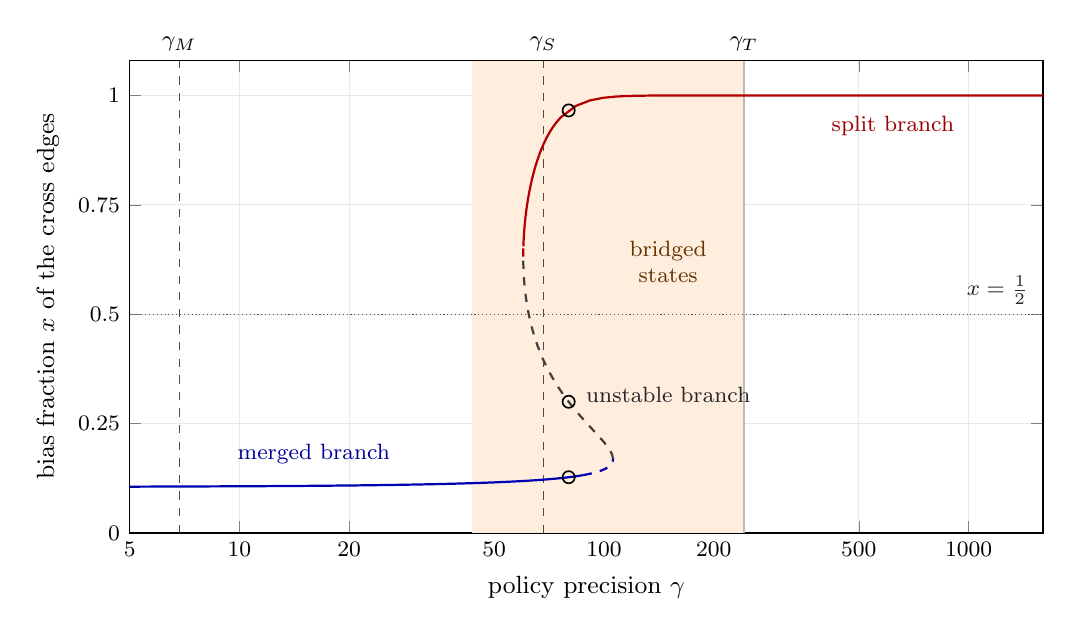
\begin{tikzpicture}
  \begin{axis}[width=11.6cm, height=6.0cm, scale only axis, xmode=log, xmin=5, xmax=1600, ymin=0, ymax=1.08,
      xtick={5,10,20,50,100,200,500,1000}, xticklabels={5,10,20,50,100,200,500,1000}, ytick={0,0.25,0.5,0.75,1},
      grid=major, grid style={gray!18},
      xlabel={policy precision $\gamma$}, ylabel={bias fraction $x$ of the cross edges},
      every axis label/.style={font=\small}, tick label style={font=\footnotesize}, clip=false]
    \fill[orange!13] (axis cs:43.41,0) rectangle (axis cs:240.98,1.08);
    \fill[gray!55] (axis cs:240,0) rectangle (axis cs:244,1.08);
    \draw[gray!60!black, dashed] (axis cs:6.845,0) -- (axis cs:6.845,1.08);
    \draw[gray!60!black, dashed] (axis cs:68.15,0) -- (axis cs:68.15,1.08);
    \draw[gray!60!black, densely dotted] (axis cs:5,0.5) -- (axis cs:1600,0.5);
    \addplot[blue!70!black, thick] coordinates {(5,0.10577) (10.707,0.10676) (16.108,0.10775) (21.22,0.10873) (26.06,0.10972) (30.643,0.11071) (34.983,0.1117) (39.094,0.11268) (42.988,0.11367) (46.677,0.11466) (50.172,0.11565) (53.483,0.11664) (56.621,0.11762) (59.593,0.11861) (62.409,0.1196) (65.078,0.12059) (67.605,0.12157) (70,0.12256) (72.267,0.12355) (74.415,0.12454) (76.448,0.12552) (78.373,0.12651) (80.194,0.1275) (81.917,0.12849) (83.548,0.12948) (85.089,0.13046) (86.546,0.13145) (87.922,0.13244)};
    \addplot[blue!70!black, thick, dashed] coordinates {(87.922,0.13244) (91.439,0.13526) (94.413,0.13807) (96.913,0.14089) (99,0.14371) (100.73,0.14652) (102.13,0.14934) (103.27,0.15216) (104.16,0.15497) (104.83,0.15779) (105.32,0.16061) (105.65,0.16342) (105.83,0.16624) (105.89,0.16906)};
    \addplot[gray!50!black, thick, dashed] coordinates {(105.89,0.16906) (105.31,0.1789) (103.89,0.18875) (101.97,0.19859) (99.765,0.20844) (97.425,0.21828) (95.046,0.22813) (92.692,0.23797) (90.401,0.24782) (88.201,0.25767) (86.103,0.26751) (84.117,0.27736) (82.244,0.2872) (80.484,0.29705) (78.834,0.30689) (77.291,0.31674) (75.849,0.32658) (74.504,0.33643) (73.251,0.34627) (72.084,0.35612) (70.998,0.36596) (69.989,0.37581) (69.051,0.38565) (68.18,0.3955) (67.373,0.40534) (66.625,0.41519) (65.932,0.42503) (65.292,0.43488) (64.701,0.44473) (64.156,0.45457) (63.655,0.46442) (63.195,0.47426) (62.774,0.48411) (62.39,0.49395) (62.041,0.5038) (61.725,0.51364) (61.441,0.52349) (61.187,0.53333) (60.961,0.54318) (60.763,0.55302) (60.591,0.56287) (60.445,0.57271) (60.323,0.58256) (60.224,0.5924) (60.149,0.60225) (60.095,0.6121) (60.064,0.62194) (60.053,0.63179)};
    \addplot[red!70!black, thick, dashed] coordinates {(60.053,0.63179) (60.057,0.63761) (60.068,0.64343) (60.086,0.64925) (60.111,0.65507)};
    \addplot[red!70!black, thick] coordinates {(60.111,0.65507) (60.183,0.66686) (60.284,0.67866) (60.414,0.69046) (60.573,0.70225) (60.762,0.71405) (60.98,0.72585) (61.229,0.73765) (61.51,0.74944) (61.824,0.76124) (62.173,0.77304) (62.559,0.78484) (62.986,0.79663) (63.455,0.80843) (63.971,0.82023) (64.539,0.83203) (65.165,0.84382) (65.858,0.85562) (66.626,0.86742) (67.483,0.87922) (68.445,0.89101) (69.536,0.90281) (70.786,0.91461) (72.244,0.92641) (73.978,0.9382) (76.107,0.95) (83.76,0.9763) (91.55,0.98877) (99.412,0.99467) (107.32,0.99748) (115.24,0.9988) (123.18,0.99943) (131.12,0.99973) (139.07,0.99987) (147.02,0.99994) (154.97,0.99997) (162.92,0.99999) (170.87,0.99999) (178.82,1) (186.77,1) (194.72,1) (202.67,1) (210.62,1) (218.57,1) (226.52,1) (234.47,1) (242.42,1) (250.37,1) (258.32,1) (266.27,1) (274.22,1) (282.17,1) (290.12,1) (298.08,1) (306.03,1) (313.98,1) (321.93,1) (329.88,1) (337.83,1) (371.61,1) (457.79,1) (563.95,1) (694.73,1) (855.84,1) (1054.3,1) (1298.8,1) (1600,1)};
    \addplot[only marks, mark=o, mark size=2.2pt, black, semithick] coordinates {(80,0.1274) (80,0.2999) (80,0.9659)};
    \node[font=\footnotesize, anchor=south] at (axis cs:6.845,1.08) {$\gamma_M$};
    \node[font=\footnotesize, anchor=south] at (axis cs:68.15,1.08) {$\gamma_S$};
    \node[font=\footnotesize, anchor=south] at (axis cs:242,1.08) {$\gamma_T$};
    \node[font=\footnotesize, blue!60!black, anchor=south] at (axis cs:16,0.135) {merged branch};
    \node[font=\footnotesize, red!60!black, anchor=north] at (axis cs:620,0.975) {split branch};
    \node[font=\footnotesize, gray!30!black, anchor=west] at (axis cs:84,0.315) {unstable branch};
    \node[font=\footnotesize, orange!40!black, align=center] at (axis cs:150,0.62) {bridged\\states};
    \node[font=\footnotesize, gray!30!black, anchor=south east] at (axis cs:1550,0.5) {$x=\frac12$};
  \end{axis}
\end{tikzpicture}

  \caption{\textbf{Mean-field phase diagram at the base point.} Symmetric fixed points of the map \eqref{eq:frm-meanfield} under \cref{asm:frm-mean-field}, shown as the bias fraction $x$ of the cross edges against the policy precision $\gamma$ and computed with the exact set softmax over the $35$ attended sets. The merged branch (blue) and the split branch (red) are joined by an unstable middle branch through folds at $\gamma=105.9$ and $\gamma=60.05$. Curves are solid where both multipliers of \cref{thm:frm-formation}(d) lie below one and dashed where one of them exceeds one, so the merged branch loses stability to symmetry-breaking perturbations at $\gamma=87.9$, before its fold. Circles mark the three fixed points at $\gamma=80$ of \cref{tab:frm-thresholds}, $x=0.1274$, $0.2999$ and $0.9659$. Dashed vertical lines mark $\gamma_M=6.84$ and $\gamma_S=68.2$ of \eqref{eq:frm-thresholds}, and the gray bar marks the global-split threshold $\gamma_T$, which lies between $240$ and $244$. Bridged states (\cref{obs:frm-bridged}), stable fixed points of the per-receiver map with one to three of the four cross edges learned, exist in the shaded range $43.4<\gamma<241.0$, whose upper end is the fold of the single learned bridge.}
  \label{fig:frm-phase}
\end{figure}
% src: figure supplied with the section; continuation values verified by the integrator (folds, symmetry breaking at 87.92, bridged range 43.41 to 240.98)

\begin{table}[tb]
\centering
\caption{Symmetric fixed points of the mean-field map at the base point: bias fraction $x$ of the cross edges with the cross attention per edge in parentheses, and the symmetric and symmetry-breaking multipliers. Classes refer to the symmetric subspace. Off it, the merged point is unstable to symmetry-breaking perturbations for $87.9<\gamma<105.9$, and bridged states exist for $43.4<\gamma<241.0$ (\cref{obs:frm-bridged,fig:frm-phase}).}
\label{tab:frm-thresholds}
\begin{tabular}{@{}llll@{}}
\toprule
$\gamma$ & fixed points $x$ (cross attention) & multipliers & class \\
\midrule
5 to 60 & $0.106$ to $0.119$ ($0.43$ to $0.37$) & $0.953$ to $0.981$ & merged only \\
80 & $0.127$ ($0.344$) & $0.976$, $0.994$ & bistable \\
 & $0.300$ ($0.117$) & $1.014$, $1.027$ (unstable) & \\
 & $0.966$ ($1.8\times10^{-3}$) & $0.995$, $0.995$ & \\
120 & $0.9992$ ($3.9\times10^{-5}$) & $0.995$, $0.995$ & split \\
160 to 1600 & $1.0000$ ($9.0\times10^{-7}$ to $2\times10^{-65}$) & $0.995$, $0.995$ & split \\
\bottomrule
\end{tabular}
\end{table}

\begin{observation}[Bridged states]\label{obs:frm-bridged}
Off the symmetric subspace the map has stable fixed points in which a receiver keeps $n_{\mathrm b}$ of its $n$ cross edges learned and attended. At the base point, continuation in $\gamma$ of the states found at $\gamma=80$ gives them for $43.4<\gamma<241.0$: $n_{\mathrm b}=3$ from its fold at $\gamma=43.41$ to $111.3$, $n_{\mathrm b}=2$ from $46.69$ to $151.2$ and $n_{\mathrm b}=1$ from $51.54$ to its fold at $240.98$, where the last learned bridge collapses, while the merged state, $n_{\mathrm b}=4$, is stable up to $\gamma=87.9$. Bridged states thus exist already below $\gamma=60.05$, where the split branch begins on the symmetric subspace, and none is found above $\gamma=241.0$ or, by iteration from bridged starts, at any $\gamma$ from $400$ to $3200$. Bridges must be nucleated: at $\gamma=160$ an edge started at $x\le0.1$ stays learned and one started at $x\ge0.2$ collapses. One reciprocal bridge per receiver at $\gamma=160$ gives group contrast $4.51$ and union contrast $1.76$, from the isotropic part of a covariance that departs by $0.44$ in relative norm from blocks proportional to $I_2$, so these values are indicative only (\cref{chk:frm-bridged}).
\end{observation}
% src: B2-X1 (refines L3-C1); C2-4 bridge survival; scalar-reduction residual from B2_bridges output; stable ranges by continuation (figure fig:frm-phase, recomputed with B2_meanfield imported read-only: folds 43.41 and 240.98, stability ends 111.33, 46.69, 151.24, 51.54)
A learned bridge persists because it is the only near-equal alternative to the in-group senders. Bridged states are what flattening leaves out: their attended subgraph is flat, but no unattended cut separates the groups.

\subsection{Baseline convention, parameter grid and finite policy precision}\label{sup:frm-baseline-convention-parameter-grid-and-f}

\begin{remark}[A weaker convention: the matched-size baseline]\label{rem:frm-matched-baseline}
The weaker convention of \cref{rem:col-baseline-conventions}, which compares a region only with regions of its own size, gives $r_{\mathrm{hom}}(n)=1$ here (\cref{thm:frm-split-contrast}(b)) and would admit every level above $r_{\mathrm{sub}}=2.318$. We do not use it: at such levels the comparison medium itself has qualifying regions (at level $3$, its whole population and its eight seven-member regions), so a selection there would not separate the split from a population without frames.
\end{remark}
% src: B2-T2(b), B2-P2(d) under the matched convention; C2-5, decision 11 (weaker convention only in a remark)

\begin{observation}[The parameter grid]\label{obs:frm-grid}
On the grid of 162 points with $F$ equal to $0.9$, $0.95$, $0.98$, $0.99$, $0.995$ or $0.999$, $Q=1-F^2$, $R^s\in\{0.25,1,4\}$, $R_c\in\{0.01,0.05,0.5\}$, $n\in\{2,4,8\}$ and $\kappa=n-1$, the calibration conditions of the split and of the comparison medium each have one root at every point, and both are nondegenerate. Everywhere $r_{\mathrm{sub}}<\bar r_{\mathrm{hom}}<r(A)$, the split contrast lies in $[1.24,60.5]$ and the significance between $1.009$ and $1.415$, so every window is nonempty, some narrower than one percent of the level, and by \cref{thm:frm-split-contrast}(e) every grid point lies in an open set on which the split at $\gamma=\infty$ with $\sigma_\alpha^2=0$ is a collective at admissible levels (\cref{chk:frm-baseline}).
\end{observation}
% src: B2-T2(c) grid statements (numerical, repair (v): uniqueness and nondegeneracy are numerical; existence proved in thm(d)); C2-5 grid significance; comparison-medium root and r_sub < rbar recomputed by the editor on the same grid

\begin{observation}[Exploration at finite policy precision]\label{obs:frm-exploration}
In the frozen-slow model with self-consistent calibration, the split branch at $\gamma=80$, $120$ and $160$ has group contrast $8.6763$, $8.7317$ and $8.7329$, union contrast at most $1.008$, and a diffusive precision of the form $\Sigma^{\mathrm{sc}}\otimes I_2$ to within $3.1\times10^{-14}$ after rotating group $B$ by the remaining cross error; at $\gamma=80$ only $A$ and $B$ among the 247 regions exceed $7.954$. On the merged branch no region exceeds $7.954$ at $\gamma=10$, $40$ or $80$. Treating the mean cross weight $Fk_\times\mathsf p_\times$ ($k_\times$ the gain of an attended cross message, $\mathsf p_\times$ the cross attention per edge) as a symmetric coupling estimates $r(A)\approx(1-\lambda_\perp^2)/(1-\lambda^2+2n\lambda Fk_\times\mathsf p_\times)$, $8.698$ against $8.676$ at $\gamma=80$ (\cref{chk:frm-exploration}).
\end{observation}
% src: B2-P1 (leading-order heuristic stated as an estimate); region enumeration at gamma = 80 and 10 by the editor
The split keeps its contrast while this cut coupling is small against the leak $1-\lambda^2$, and by \cref{lem:frm-attention}(a) exploration on the split branch is at most $\kappa e^{-\gamma\Delta\mathcal V(1/2)}$.

\begin{remark}[Openness at finite policy precision]\label{rem:frm-open}
\Cref{thm:frm-split-contrast}(e) proves openness at $\gamma=\infty$. At finite $\gamma$ openness is a sketch (\cref{app:frm}), whose unproved step is that near the split the errors reduce to a diffusive scalar precision of the form $\Sigma^{\mathrm{sc}}\otimes I_2$, verified at the base point (\cref{obs:frm-exploration}) and not proved; its other hypothesis, nondegeneracy of the calibration roots, is verified on the grid (\cref{obs:frm-grid}).
\end{remark}
% src: B2-T2(d) proof (sketch per C2 status item 4 and repair (v))

\subsection{Partner randomization and the placement of the nulls}\label{sup:frm-partner-randomization-and-the-placement}

\begin{observation}[Partner randomization and the other states]\label{obs:frm-partner}
At the base point, partner randomization at the matched rate of $\kappa$ partners per round, drawn uniformly from the $2n-1$ others, with idealized calibration solved at the null's own state, gives the contrasts of \cref{tab:frm-nulls} with unlearned cross translations and with translations learned at the null's attention rate. In neither does any region exceed $7.954$, and the cross-group world-conditional covariance is nonzero, so $\Omega_{\mathrm{int}}>0$ across groups. At the split, $\Omega_{\mathrm{int}}$ of a within-group pair is $0.024$, $0.140$ and $0.510$ nats over windows of two, four and eight rounds, and that of a cross-group pair is below $1.5\times10^{-14}$ (\cref{chk:frm-nulls}).
\end{observation}
% src: B2-P2(b),(c),(d) restated at admissible levels (C2-5); calibration under the null is the null's own self-consistent value (B2_contrast part (c) solves it so); region enumeration of both partner-randomization states by the editor

\begin{table}[t]
\centering
\caption{Contrasts at the base point and the regions selected at admissible levels $r_0\in(7.954,8.733]$; the split at $\gamma=80$ is selected for $r_0\le8.676$, and for $\gamma\ge160$ the contrasts equal those at $\gamma=\infty$ to four digits. In the row of the deletion and freezing nulls, the freezing null is taken with initial states that are deterministic or conditioned on (\cref{prop:frm-nulls}(a)). Dashes mark order parameters not computed.}
\label{tab:frm-nulls}
\begin{tabular}{@{}lllll@{}}
\toprule
State & $r(A)$ & $r(A\cup B)$ & $\Omega_{\mathrm{int}}$ across groups & selected \\
\midrule
Split, $\gamma=\infty$ & $8.733$ & $1.000$ & $0$ & $A$ and $B$ \\
Split, $\gamma=80$ & $8.676$ & $1.008$ & -- & $A$ and $B$ \\
Merged, $\gamma=40$ & $1.019$ & $7.801$ & -- & none \\
Deletion and freezing nulls & $1$ & $1$ & $0$ & none \\
Partner randomization, unlearned & $1.351$ & $3.953$ & positive & none \\
Partner randomization, learned & $1.004$ & $7.868$ & positive & none \\
Comparison medium & $1.000$ & $7.954$ & -- & none \\
\bottomrule
\end{tabular}
\end{table}

Two remarks place these comparisons within \cref{def:agy-nulls}; the second, on the explanation nulls, is in \cref{sup:frm-explanation-nulls-and-merged-regimes}. Of the remaining nulls of type D, $\mathfrak N_{\mathrm{eff}}$ and $\mathfrak N_{\mathrm{inf}}$ are not applicable, since the model has no acts, and the habit null $\mathfrak N_{\mathrm{hab}}$ is applicable and coincides with partner randomization redrawn every round with learned translations, because at $\gamma=0$ with the uniform habits of \cref{def:frm-two-group}(iv) each receiver draws its $\kappa$ senders uniformly. For partner randomization redrawn every round the stationary second moments of the null, and with them the contrast of every region, are deterministic; the test of \cref{prop:agy-tests}(b) with the largest contrast of a region as its statistic then has $p=1/(n_{\mathrm{null}}+1)$, because that contrast is larger at the split ($8.733$ at $\gamma=\infty$ and $8.676$ at $\gamma=80$ against at most $7.868$), and it rejects at level $\alpha_{\mathrm{pr}}$ when $n_{\mathrm{null}}\ge1/\alpha_{\mathrm{pr}}-1$. Partner randomization drawn once, under which the selected partition is random, and the test on contrasts estimated from finite samples are not computed.

\subsection{Reachability in the full model}\label{sup:frm-reachability-in-the-full-model}

In the runs of \cref{obs:frm-online,tab:frm-online}, early uniform attention lets cross translations be learned before calibration registers the mismatch, calibration noise acts as exploration, and at large $\gamma$ an in-group edge with an unlucky high estimate is dropped and never sampled again, its slot going to a cross edge (\cref{chk:frm-online}). The counts are not monotone in $\alpha_{\mathrm{cal}}$ at $\gamma=160$, where the rise from 2 to 7 and the fall to 1 exceed the sampling error of eight replicates (two-sided Fisher exact tests, $p=0.04$ and $0.01$, uncorrected for the number of comparisons); the remaining differences between nonzero cells, and the differences between reruns of a cell, do not.

\subsection{Abundant capacity and the grounding tension}\label{sup:frm-abundant-capacity-and-the-grounding-tens}

\begin{proposition}[Abundant capacity]\label{prop:frm-capacity}
If $\kappa\ge n$, every receiver attends at least $\kappa-n+1$ cross senders in every round at every $\gamma$, so no attention cut separates the groups. Let calibrated precisions have the frozen form of \cref{asm:frm-mean-field}(a), with any constants $\hat\sigma^2_{\mathrm{in}}>0$ and $D_{\mathrm{cal}}>0$. Then at $\gamma=\infty$ with noiseless angle observations, $\sigma_\alpha^2=0$, from the declared start, each receiver attends in every round the $\kappa-n+1$ cross senders it chose by tie-breaking in the first round, and their bias fractions converge to $\mathsf p^\ast/(\mathsf p^\ast+1)$, which is below $\frac12$ exactly when $\mathsf p^\ast<1$: for $\mathsf p^\ast<1$ they become learned bridges, and for $\mathsf p^\ast\ge1$ they stay attended without being learned.
\end{proposition}
% src: B2-P3 (first statement derived; the bridge statement derived here for the realized dynamics with sigma_alpha = 0, not for the mean-field map, whose symmetric tie persists)
Proof in \cref{app:frm}. With reciprocal learned bridges at $\kappa=n=4$ the group contrast is $2.46$ and the union's $5.14$, against $8.73$ and $1.00$ at $\kappa=n-1$ (\cref{chk:frm-capacity}). Scarce capacity is needed as in the static withdrawal threshold of \cref{thm:coh-withdrawal}.

\begin{remark}[The grounding tension in formation]\label{rem:frm-grounding}
For $\kappa=n-1$ the split contrast is $(1-\lambda_\perp^2)/(1-\lambda^2)$, whose denominator, the leak $1-F^2(1-k^s)^2$, shrinks as the sensing gain $k^s$ falls, while the withdrawal signal $D_{\mathrm{cal}}$ of \cref{lem:frm-calibration} vanishes linearly with $k^s$. Weak grounding therefore tends to raise contrast and weakens the signal that forms the cut: at $F=0.99$, raising $R^s$ from $1$ to $4$ raises the split contrast from $8.73$ to $14.33$, lowers $D_{\mathrm{cal}}/\hat\sigma^2_{\mathrm{in}}$ from $4.16$ to $1.41$ and raises $\gamma_S$ from $68$ to $154$ (\cref{chk:frm-grounding}). High-contrast collectives of weakly grounded members need higher policy precision to form, which is \cref{asm:int-a11}, the grounding tension of \cref{thm:coh-grounding-tension}, seen from the formation side.
\end{remark}
% src: B2-R2 (formula derived; numbers checked); gamma_S at R^s = 4 recomputed by the editor

\subsection{Further conjecture and open problems}\label{sup:frm-further-conjecture-and-open-problems}

\begin{conjecture}[Drifting frames survive exact fusion]\label{conj:frm-drifting-frames}
Let the group frames of the two-group model drift, the frame angles of $A$ and $B$ performing independent random walks, so that true cross translations change while in-group translations stay the identity. Then on an open set of parameters the split is selected at an admissible level under the exact-fusion null: it survives that null.
\end{conjecture}
% src: B2-C1 (B2-O4)
The uncomputed basis is that an exact-fusion receiver that rarely attends a cross edge has a broad posterior over its translation, and a Gaussian message read through a rotation of unknown angle with spread $\mathsf v$ loses information about $\eta$ by an amount positive and increasing in $\mathsf v$. An instance with drifting frames in which exact-fusion receivers attend cross edges at the merged rate at every $\gamma$ would refute it.

\begin{openproblem}[Online calibration]\label{open:frm-online}
With C1g calibration learned online, give conditions on $(\alpha,\alpha_{\mathrm{cal}},\gamma,\mathsf p^\ast)$ and on the rule for unattended edges under which the split is reached from the symmetric start with probability tending to one as the gains vanish, or show that bridged states keep positive probability.
\end{openproblem}
% src: B2-O2

\begin{openproblem}[Self-consistent calibration along trajectories]\label{open:frm-self-consistent}
Replace the frozen constants of \cref{asm:frm-mean-field} by bounds uniform over configurations, so that \cref{thm:frm-formation}(b) holds for the self-consistent mean field along whole trajectories.
\end{openproblem}
% src: B2-O3

\begin{openproblem}[Access, heterogeneity and geometry]\label{open:frm-access}
Extend the analysis to anisotropic access, where a cut can separate complementary information, to heterogeneous senders, and to groups on a graph with geometry, where contrast meets the second-moment length $\xi_2$ and the largest extent $\Lstar$ of hypothesis H4 (the question of \cref{open:sca-endogenous}).
\end{openproblem}
% src: B2-O5; L4-O8 (not answered: the model has no geometry)

\subsection{Moment bound and contrast conventions}\label{sup:frm-moment-bound-and-contrast-conventions}

\begin{remark}[The moment bound holds on every path]\label{rem:frm-moment-bound}
After the first round every realization of \eqref{eq:frm-error} has block row sums $F(1-k^s_i)\le F(1-k^s_{\min})<1$, with $k^s_{\min}=1/(R^s(1/Q+1/R^s+\kappa/R_c))$, because rotations have norm one (\cref{app:frm}). Row-sum contraction (C$_r$) and the uniform form of the moment bound (M) of \cref{asm:sca-standing} therefore hold on every path, and no cycle amplifies in the sense of \cref{thm:coh-amplification}.
\end{remark}
% src: B2-R1

\begin{remark}[Second moments and two-dimensional errors]\label{rem:frm-conventions}
As \cref{def:col-contrast} declares, contrast is computed from the scalar precision $(\Sigma^{\mathrm{sc}})^{-1}$ when the world-conditional covariance has the per-coordinate form $\Sigma^c=\Sigma^{\mathrm{sc}}\otimes I_2$ (agent indices first), and from second moments when the conditional law is a Gaussian mixture, as it is here for $\kappa<n-1$. At finite $\gamma$ the mistranslation forcing also makes the conditional covariance depend on the world path, so we use $\Sigma^c=\E[\Cov(e(t)\mid\eta)]$. For other two-dimensional states contrast is not defined, and reported numbers name the reduction used.
\end{remark}
% src: C2-5 smaller points; repair (ii); def:col-contrast already declares both conventions

\subsection{Explanation nulls and merged regimes}\label{sup:frm-explanation-nulls-and-merged-regimes}

The explanation nulls limit attribution. The world-and-access null predicts no partition, since all agents sense alike. The code null predicts the frame classes $\{A,B\}$: above $\gamma_T$ the partition is predictable from the codes alone and communication adds the contrast, while between $\gamma_S$ and $\gamma_T$ split and bridged states coexist for the same codes, and stable merged states as well up to $\gamma=87.9$ (\cref{fig:frm-phase}). Under \cref{def:agy-nulls} the split above $\gamma_T$ is therefore code aligned.

Each failure of formation in the two-group model (\cref{sec:frm-fails}) marks a hypothesis the positive results need. For $\gamma<\gamma_M$ every cross translation is learned. At the base point the symmetric map is merged only up to its fold at $\gamma=60.05$, while bridged states of the per-receiver map, found by continuation, appear already at $\gamma=43.4$ (\cref{obs:frm-bridged}); at the smaller mismatch $\vartheta=\pi/4$, where $\Delta\mathcal V(\frac12)$ is smaller, the symmetric map is merged only up to $\gamma\approx80$. A C0 receiver that assigns every sender the same noise attends uniformly (\cref{prop:coh-c0-blind}), $\mathsf p_j=\kappa/(2n-1)$, so by \eqref{eq:frm-meanfield} every cross translation ends learned whenever $\kappa/(2n-1)>\mathsf p^\ast$. Two failures are structural (\cref{prop:frm-capacity,prop:frm-exact-fusion}).

\subsection{Remarks on the formation conjecture}\label{sup:frm-remarks-on-the-formation-conjecture}

Regarding \cref{conj:frm-formation}, in the two-group model the attention and learning statements of the first two regimes hold for the frozen-calibration mean-field map (\cref{thm:frm-formation}) and the third is observed (\cref{obs:frm-bridged}). A population of this class in which, for arbitrarily large $\gamma$, a stable configuration keeps a learned and attended cross-class edge would refute the conjecture; where it holds, its collectives are attributed to misreading unless they survive exact fusion. Linear conformity to a self-constituted prior cannot form collectives (\cref{prop:hie-conformity}); a route that does not rest on misreading, through conformity of codes with member-written code records and a pragmatic coordination value, is stated as \cref{conj:hie-conformity-formation}.
